% Created by tikzDevice version 0.10.1 on 2016-09-28 15:33:03
% !TEX encoding = UTF-8 Unicode
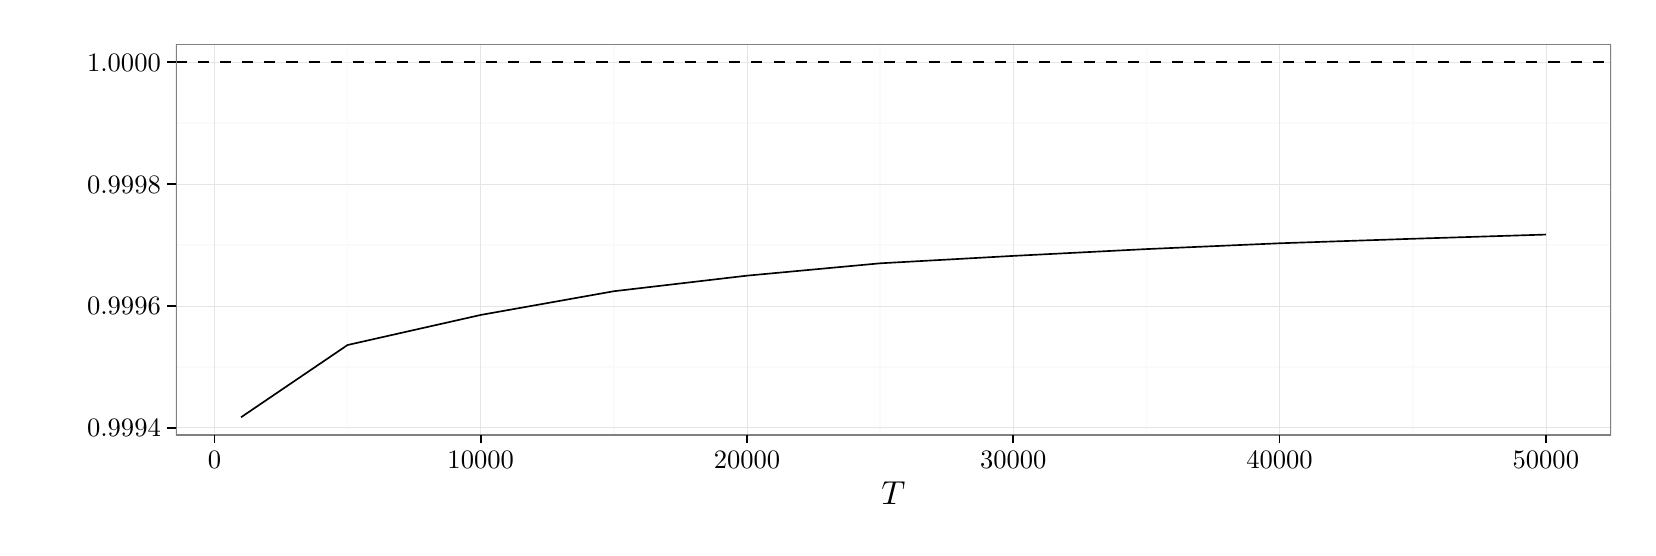
\begin{tikzpicture}[x=1pt,y=1pt]
\definecolor{fillColor}{RGB}{255,255,255}
\path[use as bounding box,fill=fillColor,fill opacity=0.00] (0,0) rectangle (578.16,180.67);
\begin{scope}
\path[clip] (  0.00,  0.00) rectangle (578.16,180.67);
\definecolor{drawColor}{RGB}{255,255,255}
\definecolor{fillColor}{RGB}{255,255,255}

\path[draw=drawColor,line width= 0.6pt,line join=round,line cap=round,fill=fillColor] (  0.00,  0.00) rectangle (578.16,180.68);
\end{scope}
\begin{scope}
\path[clip] ( 53.52, 33.48) rectangle (572.16,174.67);
\definecolor{fillColor}{RGB}{255,255,255}

\path[fill=fillColor] ( 53.52, 33.48) rectangle (572.16,174.67);
\definecolor{drawColor}{gray}{0.98}

\path[draw=drawColor,line width= 0.6pt,line join=round] ( 53.52, 58.13) --
	(572.16, 58.13);

\path[draw=drawColor,line width= 0.6pt,line join=round] ( 53.52,102.18) --
	(572.16,102.18);

\path[draw=drawColor,line width= 0.6pt,line join=round] ( 53.52,146.23) --
	(572.16,146.23);

\path[draw=drawColor,line width= 0.6pt,line join=round] (115.59, 33.48) --
	(115.59,174.67);

\path[draw=drawColor,line width= 0.6pt,line join=round] (211.81, 33.48) --
	(211.81,174.67);

\path[draw=drawColor,line width= 0.6pt,line join=round] (308.03, 33.48) --
	(308.03,174.67);

\path[draw=drawColor,line width= 0.6pt,line join=round] (404.25, 33.48) --
	(404.25,174.67);

\path[draw=drawColor,line width= 0.6pt,line join=round] (500.47, 33.48) --
	(500.47,174.67);
\definecolor{drawColor}{gray}{0.90}

\path[draw=drawColor,line width= 0.2pt,line join=round] ( 53.52, 36.11) --
	(572.16, 36.11);

\path[draw=drawColor,line width= 0.2pt,line join=round] ( 53.52, 80.16) --
	(572.16, 80.16);

\path[draw=drawColor,line width= 0.2pt,line join=round] ( 53.52,124.21) --
	(572.16,124.21);

\path[draw=drawColor,line width= 0.2pt,line join=round] ( 53.52,168.26) --
	(572.16,168.26);

\path[draw=drawColor,line width= 0.2pt,line join=round] ( 67.48, 33.48) --
	( 67.48,174.67);

\path[draw=drawColor,line width= 0.2pt,line join=round] (163.70, 33.48) --
	(163.70,174.67);

\path[draw=drawColor,line width= 0.2pt,line join=round] (259.92, 33.48) --
	(259.92,174.67);

\path[draw=drawColor,line width= 0.2pt,line join=round] (356.14, 33.48) --
	(356.14,174.67);

\path[draw=drawColor,line width= 0.2pt,line join=round] (452.36, 33.48) --
	(452.36,174.67);

\path[draw=drawColor,line width= 0.2pt,line join=round] (548.59, 33.48) --
	(548.59,174.67);
\definecolor{drawColor}{RGB}{0,0,0}

\path[draw=drawColor,line width= 0.6pt,line join=round] ( 77.10, 39.89) --
	(115.59, 66.00) --
	(163.70, 76.86) --
	(211.81, 85.43) --
	(259.92, 91.06) --
	(308.03, 95.52) --
	(356.14, 98.20) --
	(404.25,100.66) --
	(452.36,102.76) --
	(500.47,104.39) --
	(548.59,105.91);

\path[draw=drawColor,line width= 0.6pt,dash pattern=on 4pt off 4pt ,line join=round] ( 53.52,168.26) -- (572.16,168.26);
\definecolor{drawColor}{gray}{0.50}

\path[draw=drawColor,line width= 0.6pt,line join=round,line cap=round] ( 53.52, 33.48) rectangle (572.16,174.67);
\end{scope}
\begin{scope}
\path[clip] (  0.00,  0.00) rectangle (578.16,180.67);
\definecolor{drawColor}{RGB}{0,0,0}

\node[text=drawColor,anchor=base east,inner sep=0pt, outer sep=0pt, scale=  0.96] at ( 48.12, 32.80) {0.9994};

\node[text=drawColor,anchor=base east,inner sep=0pt, outer sep=0pt, scale=  0.96] at ( 48.12, 76.85) {0.9996};

\node[text=drawColor,anchor=base east,inner sep=0pt, outer sep=0pt, scale=  0.96] at ( 48.12,120.90) {0.9998};

\node[text=drawColor,anchor=base east,inner sep=0pt, outer sep=0pt, scale=  0.96] at ( 48.12,164.95) {1.0000};
\end{scope}
\begin{scope}
\path[clip] (  0.00,  0.00) rectangle (578.16,180.67);
\definecolor{drawColor}{RGB}{0,0,0}

\path[draw=drawColor,line width= 0.6pt,line join=round] ( 50.52, 36.11) --
	( 53.52, 36.11);

\path[draw=drawColor,line width= 0.6pt,line join=round] ( 50.52, 80.16) --
	( 53.52, 80.16);

\path[draw=drawColor,line width= 0.6pt,line join=round] ( 50.52,124.21) --
	( 53.52,124.21);

\path[draw=drawColor,line width= 0.6pt,line join=round] ( 50.52,168.26) --
	( 53.52,168.26);
\end{scope}
\begin{scope}
\path[clip] (  0.00,  0.00) rectangle (578.16,180.67);
\definecolor{drawColor}{RGB}{0,0,0}

\path[draw=drawColor,line width= 0.6pt,line join=round] ( 67.48, 30.48) --
	( 67.48, 33.48);

\path[draw=drawColor,line width= 0.6pt,line join=round] (163.70, 30.48) --
	(163.70, 33.48);

\path[draw=drawColor,line width= 0.6pt,line join=round] (259.92, 30.48) --
	(259.92, 33.48);

\path[draw=drawColor,line width= 0.6pt,line join=round] (356.14, 30.48) --
	(356.14, 33.48);

\path[draw=drawColor,line width= 0.6pt,line join=round] (452.36, 30.48) --
	(452.36, 33.48);

\path[draw=drawColor,line width= 0.6pt,line join=round] (548.59, 30.48) --
	(548.59, 33.48);
\end{scope}
\begin{scope}
\path[clip] (  0.00,  0.00) rectangle (578.16,180.67);
\definecolor{drawColor}{RGB}{0,0,0}

\node[text=drawColor,anchor=base,inner sep=0pt, outer sep=0pt, scale=  0.96] at ( 67.48, 21.46) {0};

\node[text=drawColor,anchor=base,inner sep=0pt, outer sep=0pt, scale=  0.96] at (163.70, 21.46) {10000};

\node[text=drawColor,anchor=base,inner sep=0pt, outer sep=0pt, scale=  0.96] at (259.92, 21.46) {20000};

\node[text=drawColor,anchor=base,inner sep=0pt, outer sep=0pt, scale=  0.96] at (356.14, 21.46) {30000};

\node[text=drawColor,anchor=base,inner sep=0pt, outer sep=0pt, scale=  0.96] at (452.36, 21.46) {40000};

\node[text=drawColor,anchor=base,inner sep=0pt, outer sep=0pt, scale=  0.96] at (548.59, 21.46) {50000};
\end{scope}
\begin{scope}
\path[clip] (  0.00,  0.00) rectangle (578.16,180.67);
\definecolor{drawColor}{RGB}{0,0,0}

\node[text=drawColor,anchor=base,inner sep=0pt, outer sep=0pt, scale=  1.20] at (312.84,  8.40) {$T$};
\end{scope}
\end{tikzpicture}
